\documentclass[11pt,a4paper]{article}
\usepackage[slovak]{babel}
\usepackage[utf8]{inputenc}
\usepackage[T1]{fontenc}
\usepackage[pdftex]{graphicx}
\usepackage{tabularx}
\usepackage{paralist}
\usepackage[margin=20mm]{geometry}

\begin{document}
\begin{titlepage}

% \vspace*{1cm}
\begin{figure}[!h]
  \centering
  
\includegraphics[width=\linewidth]{src/logo}
\end{figure}

\vfill

\begin{center}
  \begin{Large}
    Úvod do softwarového inženýrství \\
    2015/2016 \\
  \end{Large}
  %\bigskip
  \vspace{10mm}
  \begin{huge}
    Projekt IUS - Model informačního systému \\
  \end{huge}
  %\bigskip
  \vspace{10mm}
  \begin{Large}
    \textbf{Zadanie č.~29 - Hotel}
  \end{Large}

\end{center}

\vfill

\begin{center}
  \begin{Large}
  \today
  \end{Large}
\end{center}

\vfill

\begin{large}
  Jakub Kulich (xkulic03) \hfill Brno,~29.~november~2015
\end{large}

\end{titlepage}

\section*{Zadanie}
Navrhněte IS hotelu, který by poskytoval přehled o dostupnosti pokojů, údaje o hostech, jejich pobytech v hotelu, požadavcích na služby, platby za pokoje, atd. Zákazníci mohou provádět rezervace pokojů (tím pádem musí zadat své osobní údaje). Klient si může v rámci jedné rezervace objednat více pokojů, třeba i na jiné datum. Hotelu stačí mít informace pouze o jednom klientovi, který zaštiťuje celý pobyt v hotelu (o ostatních účastnících pobytu nemusí být dostupné žádné informace). Pobyt může být vytvořen na základě rezervace, nebo k rezervaci pokoje vůbec nemusí dojít, pokud klient přijde přímo na recepci hotelu. Jednotlivé typy pokojů mají různé ceny, cena pokoje se navíc může lišit podle období (turistická sezóna), na které si klient pokoj objednává. Cena pokoje se zároveň odvíjí od toho, zda si host pokoj rezervuje dopředu, nebo až na místě. Klient si může přiobjednat k danému pobytu služby v hotelu navíc, jako např. pronájem bazénu, a to i vícekrát. IS dále bude schopen evidovat skutečně absolvované pobyty - tj. které pokoje klient od kdy do kdy obýval a jaké služby skutečně využil (od x do x naKteremPokoji). U každého pobytu je evidováno, který zaměstnanec převzal platbu za pobyt. 
\section*{Diagram prípadov užitia}
\vfill
\begin{center}
  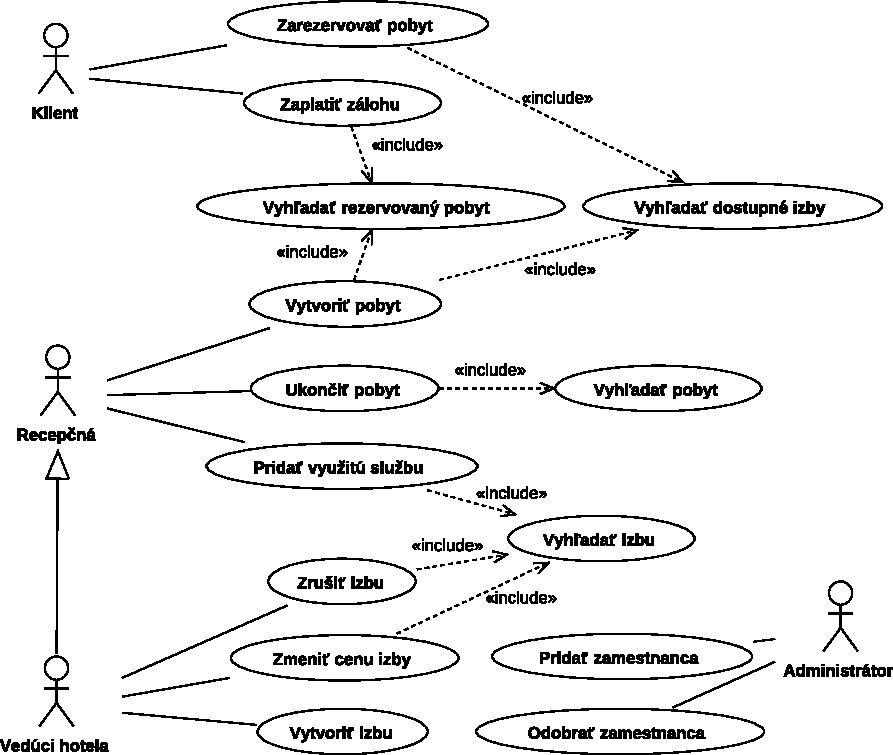
\includegraphics[width=\linewidth]{src/uc}
\end{center}
\vfill
\newpage
\section*{Detaily prípadov užitia}
\begin{center}
\begin{tabularx}{\textwidth}{| X |}
  \hline
  \textbf{Identifikátor:} UC01\\
  \hline
  \textbf{Názov:} Vytvoriť pobyt\\
  \hline
  \textbf{Popis:} Recepčná hotela \textbf{R} vytvorí klientovi \textbf{K} pobyt. \\
  \hline
  \textbf{Priorita:} 1 \\
  \hline
  \textbf{Frekvencia} Niekoľkokrát týždenne \\
  \hline
  \textbf{Vstupné podmienky:} \\
  \begin{compactenum}
  	\item Recepčná \textbf{R} je prihlásená do systému.
  \end{compactenum}\\
  \hline
  \textbf{Výstupné podmienky} \textbf{K} je ubytovaný v hoteli \\
  \hline
  \textbf{Užívatelia:} Recepčná hotela \textbf{R}\\ %,Klient \textbf{K},  Vedúci hotela \textbf{V} \\
  \hline
  \textbf{Základná postupnosť:} \\
  \begin{compactenum}
    \item Prípad užitia začína tým, že \textbf{R} vyhľadá v systéme podľa prípadu užitia \textbf{UC04}, či nemá \textbf{K} vytvorenú rezerváciu:
      \begin{compactenum}
      \item ak má, tak \textbf{R} overí či sú údaje o \textbf{K} v systéme správne. ak nie, môže ich opraviť a stav pobytu zmení z \uv{rezervácia} na \uv{pobyt}. 
        Prípad užitia pokračuje posledným krokom.
      \item ak nemá, tak prípad užitia pokračuje následujucim krokom.
      \end{compactenum}
    \item \textbf{R} vyhľadá v systéme podľa prípadu užitia \textbf{UC05} voľné izby na základe dátumu a počtu lôžok, ktoré požaduje \textbf{K}.
      \begin{compactenum}
      \item ak systém nenájde izby vyhovujúce požiadavkám, tak \textbf{R} dá možnosť \textbf{K} zmeniť požiadavky a vyhľadanie sa zopakuje.
      \item ak systém nájde izby vyhovujúce požiadavkám, tak prípad užitia pokračuje nasledujúcim krokom. 
      \end{compactenum}
    \item Systém zobrazí vyhľadané voľné izby vyhovujúce požiadavkám a zobrazí cenu jednotlivých izieb a celkovú cenu za pobyt.
    \item ak \textbf{K} s cenou a s ubytovaním súhlasí, tak \textbf{R} zadá do systému osobné údaje o \textbf{K} a potvrdí vytvorenie pobytu.
    \item \textbf{R} vykoná úkony spojené s odovzdaním izby.
  \end{compactenum}\\
  \hline
  \textbf{Alternatívna postupnosť:} \\
  \begin{compactenum}
    \item[1.-4.] \textbf{R} môže ukončiť proces vytvorenia pobytu.
  \end{compactenum}\\
  \hline

\end{tabularx}
\end{center}

\begin{center}
\begin{tabularx}{\textwidth}{| X |}
  \hline
  \textbf{Identifikátor:} UC02\\
  \hline
  \textbf{Názov:} Zarezervovať pobyt\\
  \hline
  \textbf{Popis:} Klient \textbf{K} si zarezervuje pobyt v hoteli \\
  \hline
  \textbf{Priorita:} 1 \\
  \hline
  \textbf{Frekvencia} Niekoľkokrát týždenne \\
  \hline
  \textbf{Vstupné podmienky:} \\
  %\begin{compactenum}
        %\item Klient \textbf{K} je registrovaný v systéme
  	%\item Klient \textbf{K} je prihlásený do systému
  %\end{compactenum}\\
  \hline
  \textbf{Výstupné podmienky} Klient \textbf{K} má zarezervovanú izbu (izby) v hoteli \\
  \hline
  \textbf{Užívatelia:} Klient \textbf{K} \\ %, Recepčná hotela \textbf{R}, Vedúci hotela \textbf{V} \\
  \hline
  \textbf{Základná postupnosť:} \\
\begin{compactenum}
    \item Prípad užitia začína tým, že \textbf{K} si vyberie potrebný termín rezervácie a požadovaný počet lôžok.
    \item Systém nájde podľa diagramu užitia \textbf{UC05} a zobrazí izby vyhovujúce požiadavkám spolu s cenami za 
      jednotlivé izby, ako aj s celkovou cenou.
    \item \textbf{K} si z nájdených izieb vyberie tie ktoré izby by si chcel rezervovať a potvrdením sa táto sada izieb 
      pridá do rezervácie.
    \item \textbf{K} môže ďalej:
      \begin{compactenum}
      \item pokračovať v dokončení rezervácie.
      \item zvoliť iný dátum a pridať do rezervácie ďalšiu sadu izieb (Krok 1).
      \end{compactenum}
    \item Systém potrebuje priradiť rezerváciu k nejakému kontu \textbf{K}: 
      \begin{compactenum}
      \item ak si \textbf{K} už pri nejakej predchádzajúcej rezervácií vytvoril konto, tak sa prihlási sa do svojho konta.
      \item ak konto nevlastní, vytvorí si ho zadaním osobných údajov: meno, priezvisko, adresa, telefónne číslo, e-mail.
      \end{compactenum}
    \item \textbf{K} potvrdí rezerváciu pobytu a zadané osobné údaje.
    \item Systém odošle na e-mail \textbf{K} bankové údaje na zaplatenie zálohy.
    \item \textbf{K} zaplatením zálohy potvrdí svoju rezerváciu. 
  \end{compactenum}\\
  \hline
  \textbf{Alternatívna postupnosť:} \\
  \begin{compactenum}
    \item[1.-6.] \textbf{K} môže ukončiť proces rezervácie izby.
    \item[8.] Ak \textbf{K} nezaplatí zálohu za ubytovanie do určeného termínu, systém zruší rezerváciu izieb.
  \end{compactenum}\\
  \hline
\end{tabularx}
\end{center}

\begin{center}
\centering
\begin{tabularx}{\textwidth}{| X |}
  \hline
  \textbf{Identifikátor:} UC03\\
  \hline
  \textbf{Názov:} Pridať využitú službu\\
  \hline
  \textbf{Popis:} Recepčná \textbf{R} zaznamená do systému, že \textbf{K} využil službu v hoteli. \\
  \hline
  \textbf{Priorita:} 3 \\
  \hline
  \textbf{Frekvencia} Niekoľkokrát denne \\
  \hline
  \textbf{Vstupné podmienky:} \\
  \begin{compactenum}
  	\item Recepčná \textbf{R} je prihlásená do systému.
  \end{compactenum}\\
  \hline
  \textbf{Výstupné podmienky} V systéme je zaznamenané, že klient \textbf{K} využil službu v hoteli. \\
  \hline
  \textbf{Užívatelia:} Recepčná hotela \textbf{R}\\ %Klient \textbf{K}, , Vedúci hotela \textbf{V} \\
  \hline
  \textbf{Základná postupnosť:} \\
  \begin{compactenum}
    \item Prípad užitia začína tým, že \textbf{R} vyberie zo zoznamu akú službu \textbf{K} využil.
    \item \textbf{R} vyhľadá izbu podľa prípadu užitia \textbf{UC06}. 
    \item Ďalej systém nájde na základe nájdenej izby pobyt podľa prípadu užitia \textbf{UC07}.
    \item Systém zobrazí meno \textbf{K} ktorý využíva pobyt:
      \begin{compactenum}
      \item Ak meno, ktoré \textbf{K} nahlásil sa nezhoduje s menom v systéme, tak \textbf{R} túto skutočnosť \textbf{K} 
        oznámi a prípad užitia buď končí, alebo sa vracia na krok 1.
      \item Ak nahlásené meno sa zhoduje s menom \textbf{K} v systéme, tak prípad užitia pokračuje nasledujúcim krokom.
      \end{compactenum}
    \item \textbf{R} potvrdí vybrané služby.   
    \item Systém priradí využité služby zvolenej izbe a započíta cenu služieb k cene pobytu.
  \end{compactenum}\\
  \hline
  \textbf{Alternatívna postupnosť:} \\
  \begin{compactenum}
    \item[1.-5.] \textbf{R} môže ukončiť proces pridania využitej služby.
  \end{compactenum}\\
  \hline
\end{tabularx}
\end{center}

\section*{ER diagram}
\vfill
\begin{center}
  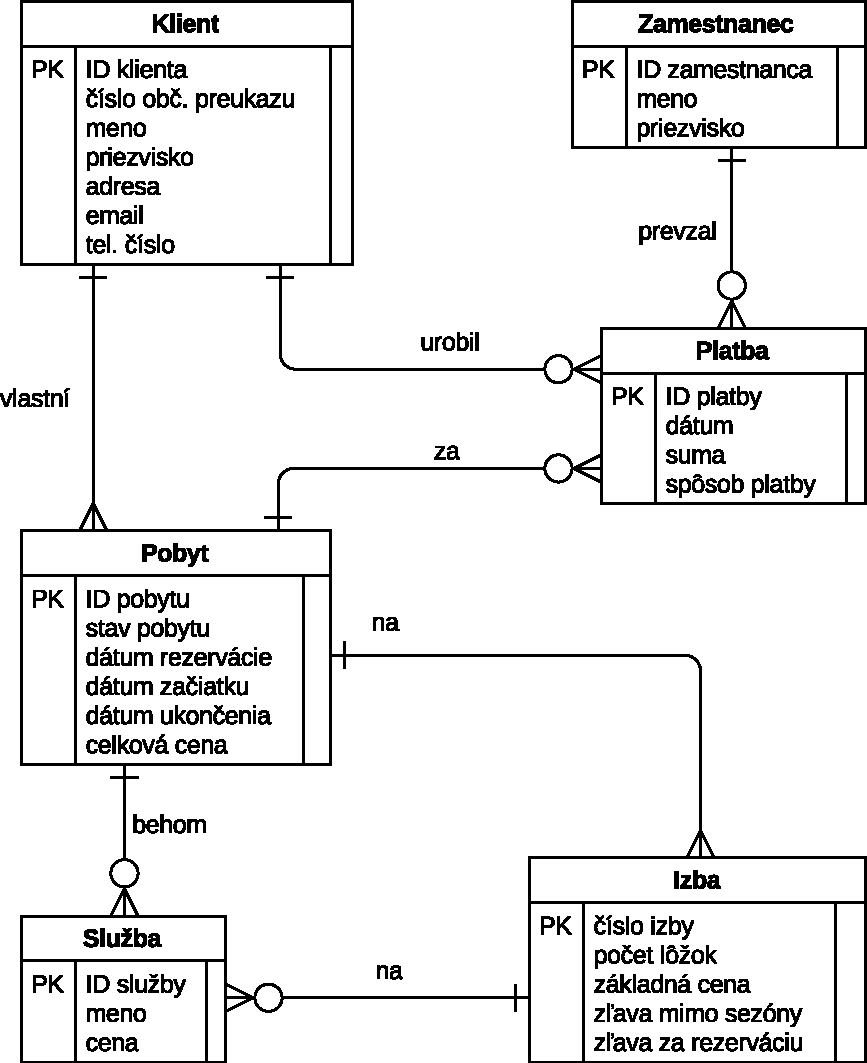
\includegraphics[width=0.7\linewidth]{src/er}
\end{center}
\vfill
\end{document}
